\documentclass[11pt]{article}

\usepackage{changepage}
\usepackage{graphicx}
\usepackage{amssymb} %math symbols
\usepackage{mathtools} %more math stuff
\usepackage{amsthm} %theorems, proofs and lemmas
\usepackage{optidef} %fast optimization problem notation
\usepackage{biblatex} %Imports biblatex package
\addbibresource{papers.bib} %Import the bibliography file

%% declaring abs so that it works nicely
\DeclarePairedDelimiter\abs{\lvert}{\rvert}%
\DeclarePairedDelimiter\norm{\lVert}{\rVert}%

\title{MICRO-453 - Boxfish robotics practical}
\author{Gabriel Vallat, Lucas Bost, Titouan Renard}

\begin{document}

\maketitle
\tableofcontents
\section{Introduction and presentation of the hardware}

\textit{TODO : explain the deal with the robot's modules and show a few pictures} 

\begin{figure}[h!]
    \centering
    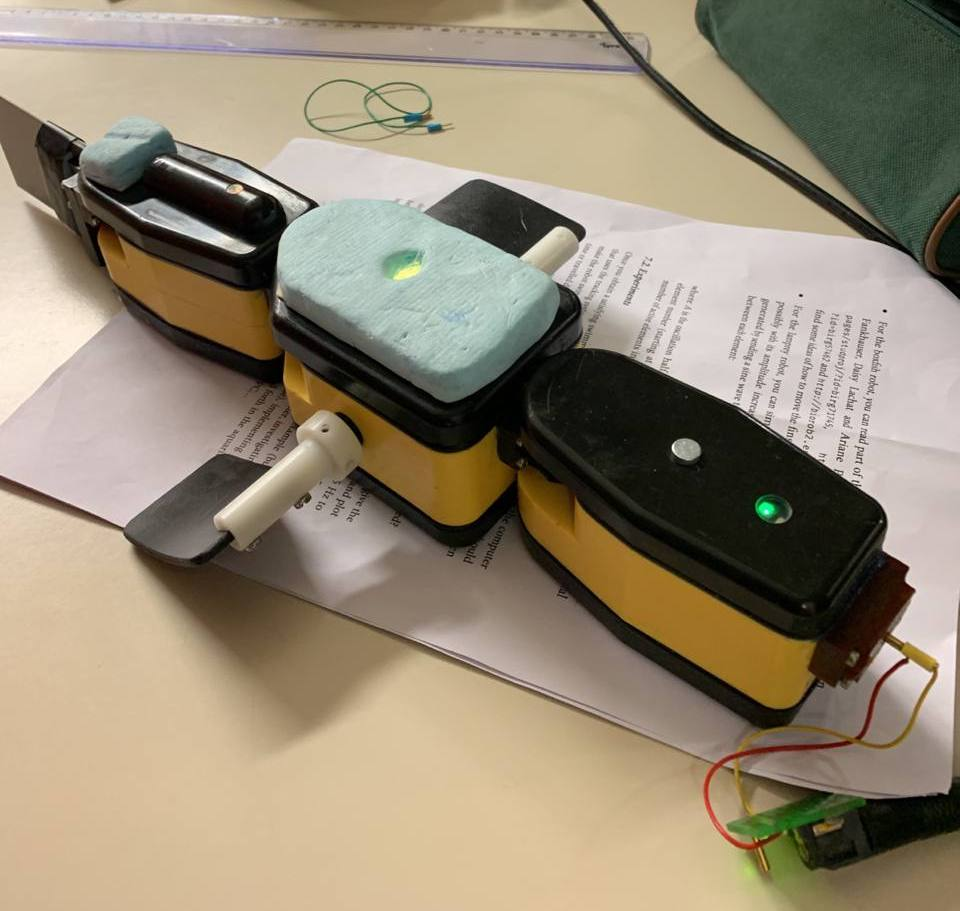
\includegraphics[width=0.8\textwidth]{figures/boxfish.jpg}
    \caption{The boxfish robot.}
    \label{boxfish}
\end{figure}

This report presents results from a practical session from the MICRO-453 course. It discusses the implementation of a simple control algorithm for a \textit{boxfish} bioinspired robot built out of \textit{salamadra robotica II} modules \cite{salamadra_robotica_2}. The robot is build of $3$ modules and has $4$ actuators.

\section{On-board and off-board software}


\subsection{Compiling and flashing the robot's microcontroller}

\textit{TODO : Point 1 (First program), 2 (Registers)}

\subsection{Internal communication between the robot's modules}

\textit{TODO : Point 3 (Communication with other elements)}

\subsection{Robot-computer radio communication}

\textit{TODO : Point 4 (Position control of a module)}

\subsection{Position tracking}

\textit{TODO : Point 6 (LED tracking system), 6.1 (Combining LED tracking system with radio)}

\section{Control of the boxfish}

\subsection{Simple onboard trajectory generation}

\textit{TODO : Point 5.1 (Simple onboard trajectory generation), 5.2 (modulating trajectory parameters)}

\subsection{Proposed swimming controller}

\textit{TODO : Point 7.1 (writing a swimming trajectory generator)}

\subsection{Proposed position controller}

\textit{TODO : Point 8 propose a PID loop on position control with waypoints ???? that would be cool anyway}

\section{Experiment}

\subsection{Optimizing the swimming gait}

\textit{TODO : Point 7.2 (influence of frequency)}

\subsection{Optimizing the position controller}

\printbibliography %Prints bibliography

\end{document}
